
\glsresetall

\newcommand{\narr}{\noindent Narrator:\\}

\mdfdefinestyle{MyShadeQuoteStyle}{%
    leftmargin=20pt,
    rightmargin=20pt,
    backgroundcolor=gray!10,
    linewidth=0pt,
    skipbelow=\topskip,
    skipabove=\topskip
}

\newenvironment{shadequote}[1][]{%
    \ignorespaces%
    \begin{mdframed}[style=MyShadeQuoteStyle,#1]%
}{%
    \end{mdframed}%
    \ignorespacesafterend%
}%

\chapter{Let Them Eat Steak: A Chapter for the Non-Scientist}
\label{ch:public}

{
\setlength{\parindent}{0pt}
\setlength{\parskip}{1em}
\setstretch{1.4}

\begin{quoting}
  {
  \footnotesize
  \textit{This chapter was written to convey my PhD work to the general public
  and was supported by the Wisconsin Initiative for Science Literacy (WISL).}
  
  \textit{This chapter is a result of me keeping a promise to myself, and so
  despite its cheesy approach to telling a tale of science, it is a beautiful
  and important moment for me. I have a lot of people to credit for helping
  bring this story from a parallel universe into reality: Anna Stephenson for
  the illustrations and helping me convert my graphics from sterile science to
  adorable art; Robin Kinchen Cenac (and Reya!) and Louise Opotowsky for
  overall creative guidance and for suffering through highly technical
  explanations of my work to prepare me for writing this chapter; Prof. Paul
  P.H. Wilson, Almost-Dr.  Kalin Keisling, Dr. Dinh Truong, and Dr. Richard
  Rojas Delgado for feedback and suggestions on my fake country names; and
  last, never least, but always the littlest, Ninjita Binjita, for the
  all-important role of lap warmer.} 
  }
\end{quoting}

\narr Welcome, curious companions! Our good friend has got a tale to tell.  But
they cannot tell this story on their own, so they asked me to give you some
background and science along the way.

\textit{Be warned: the country names are drawn from a parallel universe with
different nations and international relations. Any similarities to countries
that exist in this universe are purely coincidental. Additionally, there are
fantastical details throughout the tale, and the capability of our curious
companions to decipher between fantasy and science is presumed.  This parallel
universe also doesn't have an Earth with the same climate crisis, so the steak
in this analogy is definitely from a happy cow on a regenerative farm.}

\begin{tcolorbox}[halign=center]
\textbf{Background \& Introduction}
\end{tcolorbox}

Many underappreciated jobs keep a civilization functioning. For example,
excluding New Orleanians and other People of the Pothole (yes, New Orleans
exists in the parallel universe), you probably don't think about how you hold
the expectation that your roads are drivable. There are those responsible for
moving your garbage out of sight and mind, there are also people who clean up
roadkill, and there are those who clear the shards of a car accident with
fascinating speed. In fact, when any civic role functions well, it isn't
noticed. It is an odd result of a well-functioning society that the most
essential components remain unseen until they no longer function. Jobs like
this exist at the federal level, generally unseen, because they are so crucial
they regularly get bipartisan support. This is a story about \textit{those}
people.

Now to our friend\ldots

\begin{shadequote} 

  Imagine the scene: they were sitting in their backyard in perfect weather,
  breeze blowing, flowers flowering, and chipmunks chirping, eyes closed as the
  sun warms their skin. Suddenly they felt a chill, and opened their eyes to a
  dark sky.
  
  Except it wasn't a dark sky, it was a drone hovering over them with a package
  for delivery! C'est myst\'{e}rieux! They hadn't ordered anything. What could it 
  be? 
  
  Why, it was a package of nuclear material \textit{(Narrator: well-packaged,
  because we are not irradiating our friend)} delivered anonymously. Turns out,
  they unknowingly intercepted the attempted smuggling of nuclear material to
  construct a weapon inside the borders of United Fissions of Uranium (the
  UFU). And now our friend is officially in the middle of an international
  drama. What to do? Who to tell? 

\end{shadequote}

\begin{figure}[!htb]
  \centering
  \makebox[\textwidth][c]{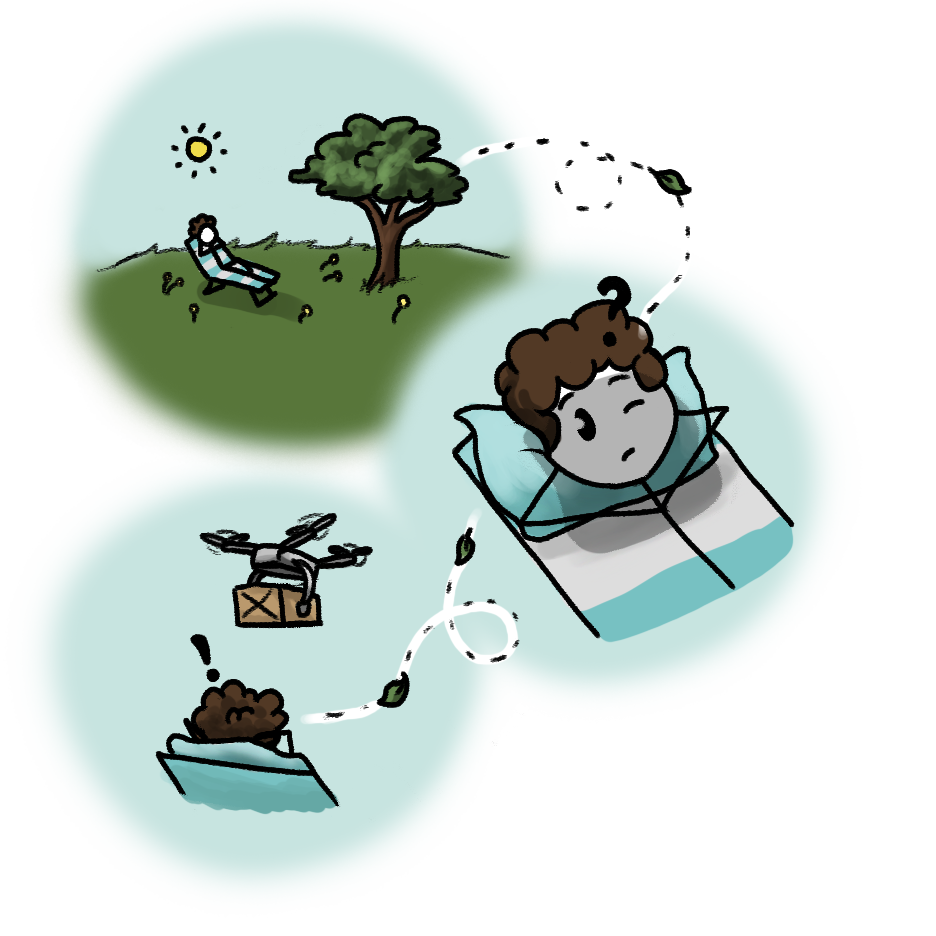
\includegraphics[width=0.9\linewidth]{./chapters/public/intro.png}}
  \large Our friend's day is quite ruined. \small Illustration by Anna Stephenson
\end{figure}

\narr I actually don't know who they should have told; federal jurisdictional
decisions for nuclear incidents is not the drama being told today. But the
authorities quickly found out and figured that out for themselves.

\begin{shadequote} 

  This turns out to be a misdelivered package, because nuclear terrorists are
  people too\ldots that sometimes make typos. The UFU authorities believe that
  there are many more packages on their way to different locations, but having
  no intel on where to intercept them, they need to know where this material
  came from to locate the terrorist group responsible. They need nuclear
  security experts, and FAST.

\end{shadequote}

\narr \textit{Enter: nuclear security}. This is not to be confused with nuclear
safety, that is, making sure nuclear power reactors behave and do not have
accidents that harm the environment and the beings in it---a more-than-worthy
effort, but not the one being discussed here. The nuclear security enterprise
instead focuses on preventing or mitigating undesirable outcomes of a different
variety, like nuclear terrorism. Nuclear security's goal is keeping all of the
nuclear material in the world inside a regulatory pipeline, so none of it gets
into the hands of people who want to do others harm.

\noindent In this universe:\\ A high profile example of nuclear security at
work, at least on a diplomatic level, is the Joint Comprehensive Plan of
Action\footnote{For more information on the JCPOA, see this
\href{https://www.armscontrol.org/factsheets/JCPOA-at-a-glance}{\color{violet}fact
sheet}}, better known as the Iran nuclear deal. Personal opinions (if you have
them) and recent news (if you've seen it) aside, its purpose is to keep a
closer eye on the country to be sure they aren't developing the capabilities
necessary to make weapons.  Another part of the nuclear security effort is a
strong nuclear forensics capability.  Nuclear forensics begins \textbf{after} a
nuclear incident occurs, which sadly, happens. This incident can be some intact
material drone-delivered to a friend by mistake, or it could be something even
worse, like the detonation of a nuclear weapon. Just in 2019, the International
Atomic Energy Agency confirmed malicious intent for six incidents of trafficked
nuclear material.

Most might think of forensics as catching a murderer, but this is more like
catching the nuclear smuggler. Given some nuclear material (a body) and
composition of the material\slash how it was encased and transported (the clues
around it like blood and fingerprints), how\slash from where was the nuclear
material obtained and\slash or smuggled (what conclusions can be drawn about
the murder)?  In both situations, forensics work ideally leads to blaming, with
court-admissible proof, someone for the illegal act. Fingerprints of humans are
important to a murder investigation, and likewise, there are fingerprints of
nuclear materials that can provide their point of origin and\slash or where
they were processed.

\begin{shadequote}

  Slight correction: They need \textbf{nuclear forensics} experts, and FAST. 
  
  These UFU authorities are in luck, since our friend happens to be a hobby
  nuclear forensics scientist! As a citizen scientist, they cannot use actual
  nuclear materials or well-equipped laboratories to test their methods and
  ideas. Our friend instead uses their software development and simulation
  skills to study their favorite topic of attributing mysterious nuclear
  materials to their point of origin. This is now their chance to unveil a
  research method to the authorities and see if they can help prevent a nuclear
  weapon from being detonated in the UFU in time. 
  
  But the authorities are not sure. Some experimental method developed by a
  \sout{grad student} hobby scientist surely wouldn't work? Also, it's not
  validated, so it wouldn't hold up in court. But the race to save lives is on.
  ``What,'' they ask, ``do ya got cookin'?''

\end{shadequote}

\narr I'll tell you all about what our friend has cookin': some steak. But hold
on, I'll get there in a minute.

From a visual inspection, the nuclear material in question has been determined
to be nuclear fuel after it's been loaded into, used in, and removed from a
nuclear reactor. By performing some to-be-discussed nuclear forensics
approaches on this material, we can figure out all of the details of this fuel
related to its creation, time in the reactor, and how long it has been out of
the reactor. 

First, I need to define some terms for you. There are four main concepts that
are covered: \textit{reactor type}, \textit{burnup}, \textit{enrichment}, and
\textit{time since irradiation}.  Ideally, the process of determining these
parameters can pinpoint a sample of nuclear fuel to the exact reactor it came
out of!

\begin{figure}[!htb]
  \centering
  \makebox[\textwidth][c]{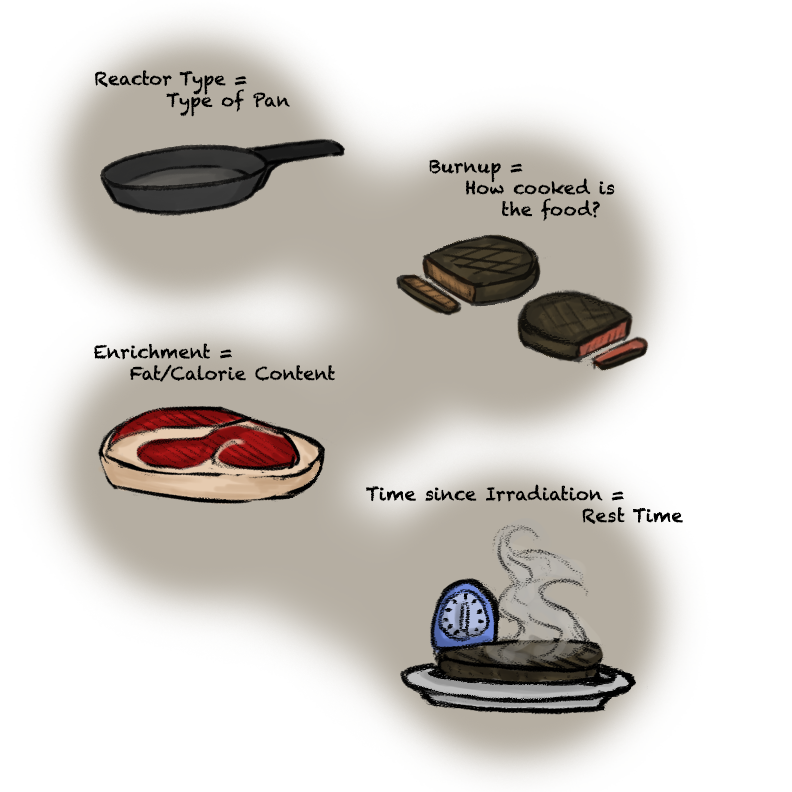
\includegraphics[width=0.9\linewidth]{./chapters/public/nukemetaphor.png}}
  \large If you imagine nuclear fuel as steak, you might be able to figure out 
  the reactor that made it! \small Illustration by Anna Stephenson
\end{figure}

Let's consider the nuclear fuel as food, specifically, steak. We can think of
the reactor as the type of pan our steak was cooked in. If it's cast iron,
it'll make a different steak than a \$10 nonstick pan that's only nonstick for
3 uses (the parallel universe shares some similar woes). The same is true for
nuclear fuel; it looks quite different depending on which reactor type it spent
time in. Our friend focuses on three main types of nuclear reactors, called
\glspl{PWR}, \glspl{BWR}, and \glspl{PHWR}\footnote{We won't cover any details
about these reactors here, but if you're curious about different types of
nuclear reactors,
\href{http://www.world-nuclear.org/uploadedFiles/org/WNA/Publications/Nuclear\_Information/Pocket\%20Guide\%20Reactors.pdf}{\color{violet}here}
is a great summary.}; different countries use one or a mix of these three main
technologies. (More than these three exist, but these are the ones our friend
wants to focus on.) 

There's also a measurement called burnup. In steak-talk, this is how well-done
it is (more accurately, it is how much energy your steak produces, but it is
more ``well-done'' as it cooks longer and produces more energy), and would be
measured in energy produced per unit of raw steak. In nuclear-talk, it's
measured in energy (mega- or gigawatt-days) per metric ton of initial uranium
(MWd/MTU or GWd/MTU). 

Next, the enrichment, meaning \% \gls{U235} enrichment, which refers to how
much of this type of uranium is in the nuclear fuel when it's freshly made.  A
lot of the time, nuclear engineers refer to a specific element from the
periodic table with a mass number attached, like \gls{U235}, as nuclides,
because the concept of nuclides emphasizes nuclear properties, which can differ
drastically even though they are the same element on the periodic table. ``U'' is
shorthand for uranium, and the mass number 235 refers to the number of protons
(92) plus neutrons (143) in the nucleus of the atom. The protons have a
positive charge, and the neutrons have no charge; the protons are balanced by
the negative charge of an equal number of electrons, but we aren't worried
about those right now. \gls{U235} is a special nuclide that nuclear engineers
call \textit{fissile}\footnote{For more information on nuclides and what
fissile means, check out this
\href{https://whatisnuclear.com/isotopes.html}{\color{violet}link}.}: when it
absorbs an extra neutron, it splits into two atoms and releases some energy.
When this energy is harnessed into our electrical grid, it's great, but that
energy can also be harnessed into a weapon, which is not great. This is like
the calorie content or fat content of your steak. The more fat, the more
calories, and so the more energy it can supply. In nuclear fuel, more fissile
material in the form of a higher \gls{U235} enrichment means that the fuel can
provide more energy than a fuel of lower enrichment. Uranium naturally has
0.7\% \gls{U235} in it, but commercial nuclear fuel is commonly enriched up to
5\%.

Last, the time since irradiation measures how long the nuclear fuel, or steak,
has been cooling after it leaves the reactor, or pan. Nuclear fuel is intensely
radioactive when it leaves the reactor, which produces a lot of heat, so it
needs to cool off for a few years to be able to be stored longer term without
heat dissipating measures (which is submerging the nuclear fuel in water; think
of the fuel as taking a several year vacation in a swimming pool). This is just
like our steak needing to rest a little before it's consumed. And that's about
as far as this metaphor can go, because aside from some recent Godzilla movies,
I don't think any of us are eating nuclear waste (in this universe, at least). 

If a nuclear material spent time in a nuclear reactor, these four parameters,
part of what we will call the reactor operation history, are important to
identifying where it came from. Next, we will talk about how identifying
where it came from can happen in an investigation.

\begin{figure}[H]
  \centering
  \makebox[\textwidth][c]{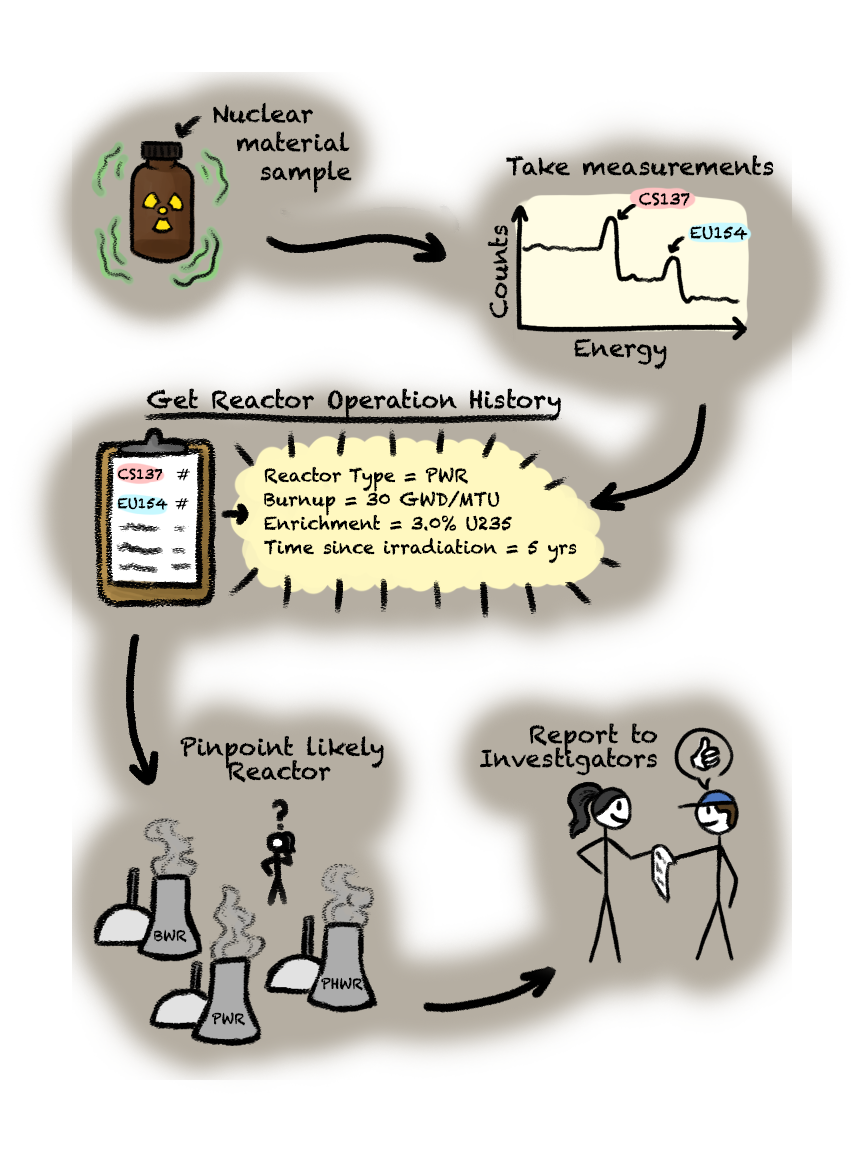
\includegraphics[width=0.8\linewidth]{./chapters/public/nf-workflow.png}}
  \large It's as simple as this $\uparrow$. \small Illustration by Anna Stephenson
\end{figure}

After some of-unknown-origin nuclear material believed to be from a reactor
enters our consciousness, some measurements will be taken by technicians
working with the government. For example, this could be something called
\textit{gamma spectroscopy}, which is pictured in the process below. This
detector measures a type of radioactivity called gamma rays\footnote{Gamma rays
are really cool, and if you read
\href{https://www.symmetrymagazine.org/article/incredible-hulking-facts-about-gamma-rays}{\color{violet}this
article}, you'll think so too!}, and gamma rays have different energies. So the
material is just sitting there spitting out gamma rays left and right and up
and down and the detector is just sitting there measuring the ones that hit it.
It collects counts of gamma rays associated with an energy; this is called a
gamma spectrum. Gamma rays of certain energies are known to come from certain
nuclides. 

Knowing how much of certain radioactive nuclides is in a material can
tell us about the reactor operation history: the reactor type (pan), burnup
(doneness), enrichment (fat), and time since irradiation (rest time). After
determining these parameters, a specialist can pinpoint a specific reactor
somewhere in the world (via access to a reactor history database) that created
the material and investigators can use that to move forward with their work.

\begin{tcolorbox}[halign=center]
\textbf{Methodology}
\end{tcolorbox}

\begin{shadequote}

  In the time it took to get through the lesson above, a foe had enough time to
  arrive on the scene: an official government scientist. This scientist has a
  different priority: precision over speed. Our friend's research is driven by
  ``how fast can I get an answer?'', whereas the scientist is driven by
  ``what's the most correct answer?'' These two priorities in this situation
  are at odds, but both equally important. The authorities need an answer, and
  fast, but it needs to be the right one because otherwise many UFU lives are
  at risk.
  
  Our friend was in the middle of telling the authorities about their fast
  nuclear fuel-identifying machine learning approach when this scientist
  arrived, so they got to listen in:
  
  ``Machine learning is a field under the umbrella of artificial intelligence,
  which allows computers to imitate human behavior. Scientists are using
  machine learning in many fields to solve complex problems, and so I wanted to
  see if it could be useful in my favorite area of study: nuclear forensics.''
  
  Pointing to the top of the diagram, they say, ``So, I first simulated hundreds
  of thousands of examples of nuclear fuel scenarios: different reactor types,
  many levels of burnup, different levels of \gls{U235} enrichment, and times
  since irradiation spanning up to 16 years.  Each simulation gives me lists of
  nuclides and their measurements that are important to determining those four
  parameters.  Machine learning professionals call these lists of nuclides the
  \textit{features}, and the parameters are \textit{labels}. All together, it's
  called a \textit{training data set}.''
  
  Pointing to the middle, ``Next, this training data is put into a
  \textit{machine learning algorithm}\footnotemark[5], which is how people
  teach computers to teach themselves with some software method. Using the
  training data set, the algorithm creates a model, which is usually a model we
  can't see or understand as humans. They are quite secretive creatures, don't
  you think?  Anyway, there are many different types of algorithms, and I have
  tested out some simple ones to see if this approach is even remotely
  feasible. These also happen to be the less-secretive type of algorithms so we
  can understand what the models are doing. One seems to work really well,
  called \gls{MLL} calculations\footnotemark[6], and I think it's good enough
  to use to save UFU.''
  
  Last, they point to the bottom of the diagram. ``So now we have the model. If
  we take the same measurements that exist in the training database features,
  then we can use the model to give us a predicted label, in this case burnup.
  But because I'm doing this experimentally, I know the actual label because I
  simulated this unknown nuclear material. So in this way, I can measure the
  prediction errors and refine my method.''
  
\end{shadequote}

\begin{figure}[H]
  \centering
  \makebox[\textwidth][c]{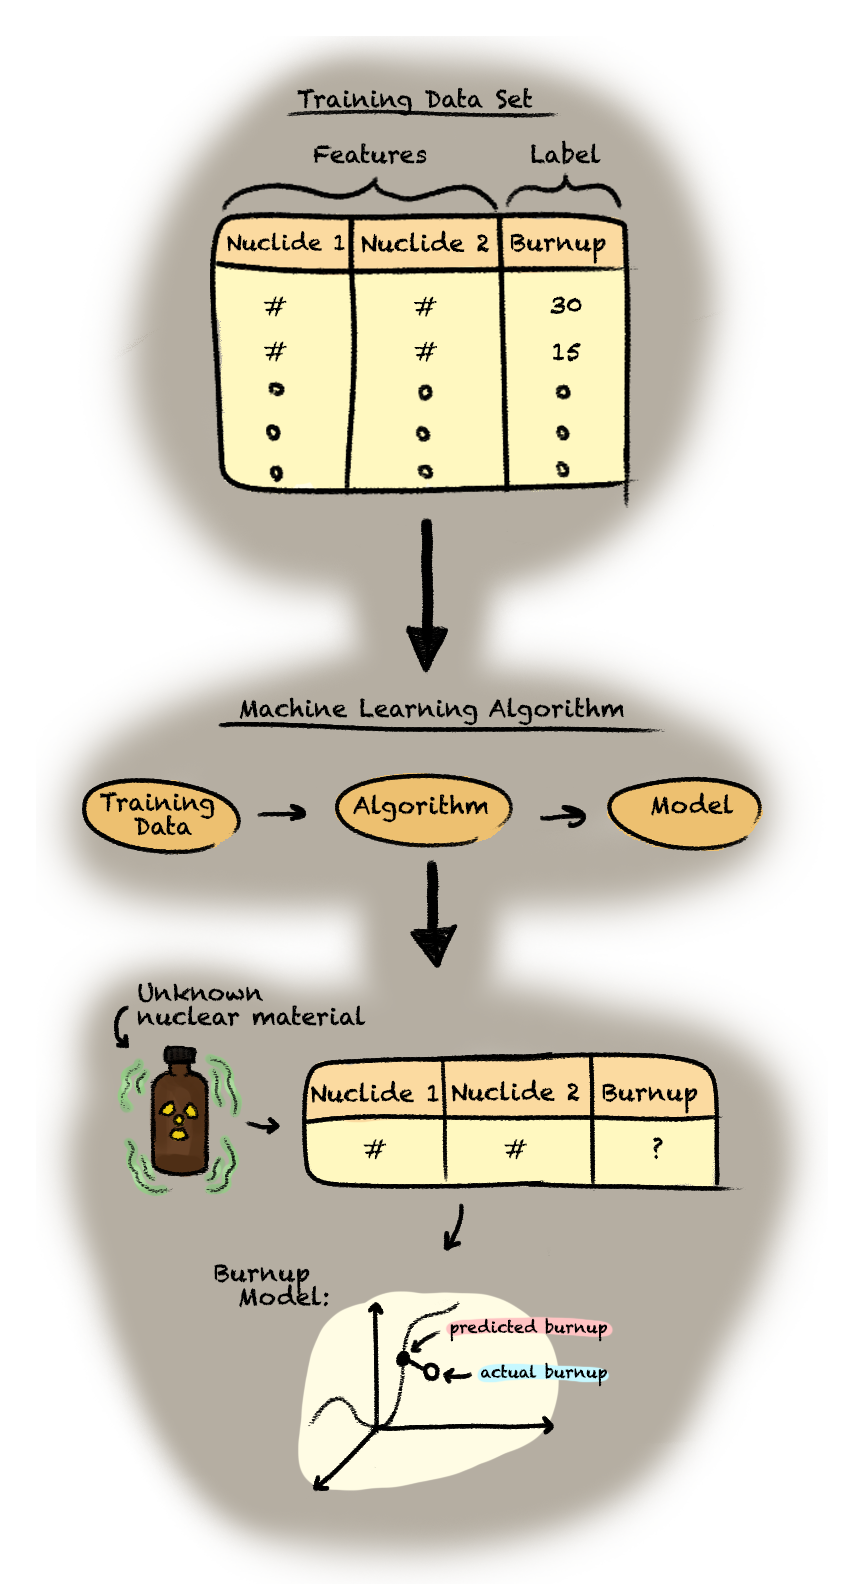
\includegraphics[height=0.9\textheight]{./chapters/public/ml-workflow.png}}
  \large Again, it's as simple as this $\uparrow$. \small Illustration by Anna Stephenson
\end{figure}

\begin{shadequote}

  The UFU authorities' eyes glazed over, but the scientist was excited. They
  were thinking, ``My oh my, we could use this! I have a database just like this
  of the most perfect simulated nuclide measurements that I can use back at the
  lab! I never really knew what to do with it, so I took a screenshot of a few
  entries and used it as my desktop background; databases are beautiful.''
  
  But our friend didn't think the scientist could take the proper measurements
  in time. Our friend uses this method with a different kind of training set,
  one that is created by simulating detectors that can take measurements in
  minutes \textit{(Narrator: remember the gamma spectroscopy from above?)},
  with the expectation that this would help in a real world scenario like this
  one. The gamma detectors measure the radioactivity of the sample, which is
  more difficult to get a direct answer from than the scientist's method in the
  lab, but our friend is all about speed. The measurements the scientist needs
  to take to match the sample with their training database involve dissolving
  the material and making many different measurements of the nuclides using a
  technique called mass spectrometry\footnotemark[7].  It gives super accurate
  results that will do well with the machine learning method, but the
  measurements take weeks. 
  
  They fought about this for about an hour, which was silly because our friend
  could have taken the gamma measurements in a fraction of that time and been
  off to use their machine learning model. But, tensions were high, egos were
  flaring, and everyone wanted to save lives. 
  
  The UFU authorities deglazed their eyes and looked at each other, then at our
  friend, then at the scientist. After some telepathic decision making, they
  said, ``We choose\ldots\ldots''

\end{shadequote}
\footnotetext[5]{For a better introduction to machine learning, read
\href{https://towardsdatascience.com/introduction-to-machine-learning-for-beginners-eed6024fdb08}{\color{violet}this}!}
\footnotetext[6]{If you have institutional access to journals,
\href{https://www.tandfonline.com/doi/full/10.1080/00295450.2017.1401442}{\color{violet}here's
the method's first paper}.}
\footnotetext[7]{I tried to find a non-company-affiliated source that explained
this simply, but failed.
\href{https://www.jeolusa.com/RESOURCES/Analytical-Instruments/Mass-Spectrometry-Basics}{\color{violet}This
is a good explanation}, though, if you're curious about mass spectrometry.}

\vspace{5mm}
\narr Now, you, curious companion, must choose your own adventure. Do we use
our friend's speedy strategy or do we trust the scientist's careful course of
action? Remember, we want to be fast, which our friend can most likely do, but
we also want to be right, which the scientist can most likely do.

\vspace{-13mm}
\begin{figure}[H]
  \centering
  \makebox[\textwidth][c]{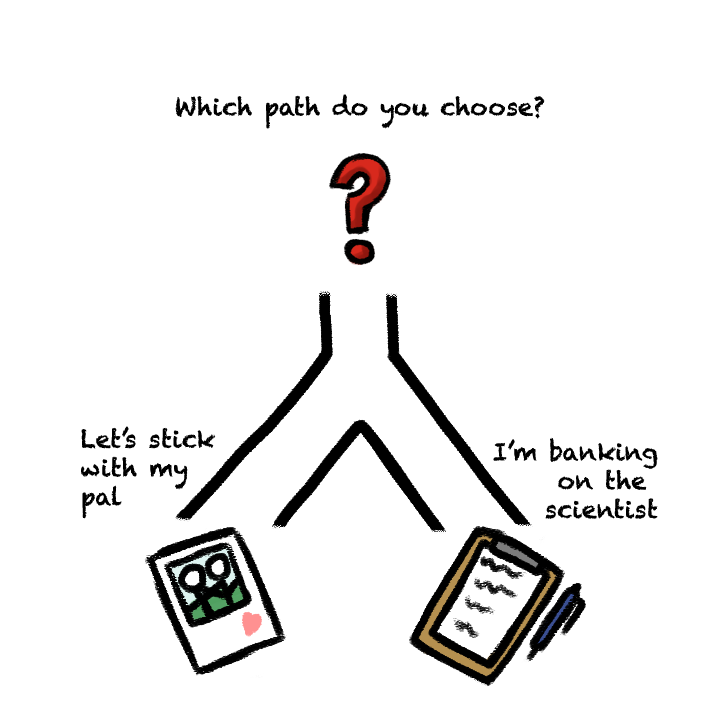
\includegraphics[width=0.69\linewidth]{./chapters/public/path.png}}
  \small Illustration by Anna Stephenson
\end{figure}
\vspace{-6mm}

\noindent \fcolorbox{gray!10}{gray!10}{
  \begin{minipage}[t]{0.45\textwidth}
    
    \setlength{\parskip}{1em}

    ``\ldots our friend!'' Now the race is on to measure the material with a
    gamma detector and predict the fuel's reactor operation history. For a
    hobbyist, our friend has a pretty great gamma detector: a portable
    high-purity germanium detector. It can detect the gamma rays very
    precisely, and our friend always wants to use the best detector they can
    get their hands on.

  \end{minipage}%
}
  \hfill\vline\hfill
\noindent \fcolorbox{gray!10}{gray!10}{
  \begin{minipage}[t]{0.45\textwidth}
  
    \setlength{\parskip}{1em}

    ``\ldots the scientist!'' Now the scientist takes the nuclear fuel to start
    making measurements. Back in their fancy state-of-the-art lab with all the
    mass spectrometry equipment a radiochemist could ever dream of, the
    scientist and their team get started. One week goes by, two weeks go by.
    And by the third week the scientist and their team had measured 29 nuclides
    in the nuclear fuel sample to high precision! 

  \end{minipage}
}

\noindent \fcolorbox{gray!10}{gray!10}{
  \begin{minipage}[t]{0.45\textwidth}
    
    \setlength{\parskip}{1em}

    \vspace{-22pt}
    \begin{figure}[H]
      \centering
      \makebox[\textwidth][c]{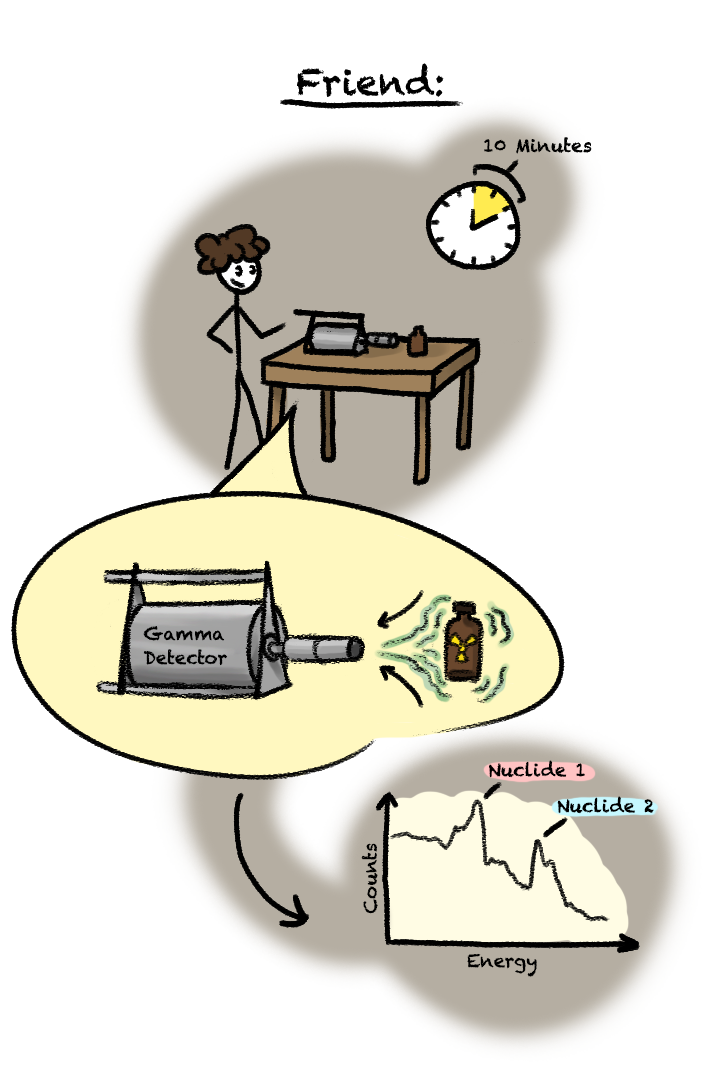
\includegraphics[width=0.95\linewidth]{./chapters/public/gamma_spec.png}}
      \large This process doesn't require advanced training. 
      \small Illustration by Anna Stephenson
    \end{figure}
    \vspace{-7mm}
    
    Using the technical assistance of the UFU authorities, our friend was able
    to protect themself against radiation and take the sample out of its
    packaging to get the best measurements possible. They let the detector
    measure the sample for 10 minutes, et voil\`{a}: a gamma spectrum of the
    sample. Our friend then took the gamma spectrum and compared it against
    their machine-learned model that was created using a training set composed
    of $450,000$ simulated gamma spectra of different types of nuclear fuel.
    And out popped an answer:
  
  \end{minipage}%
}
  \hfill\vline\hfill
\noindent \fcolorbox{gray!10}{gray!10}{
  \begin{minipage}[t]{0.45\textwidth}
  
    \setlength{\parskip}{1em}
    
    \vspace{-46pt}
    \begin{figure}[H]
      \centering
      \makebox[\textwidth][c]{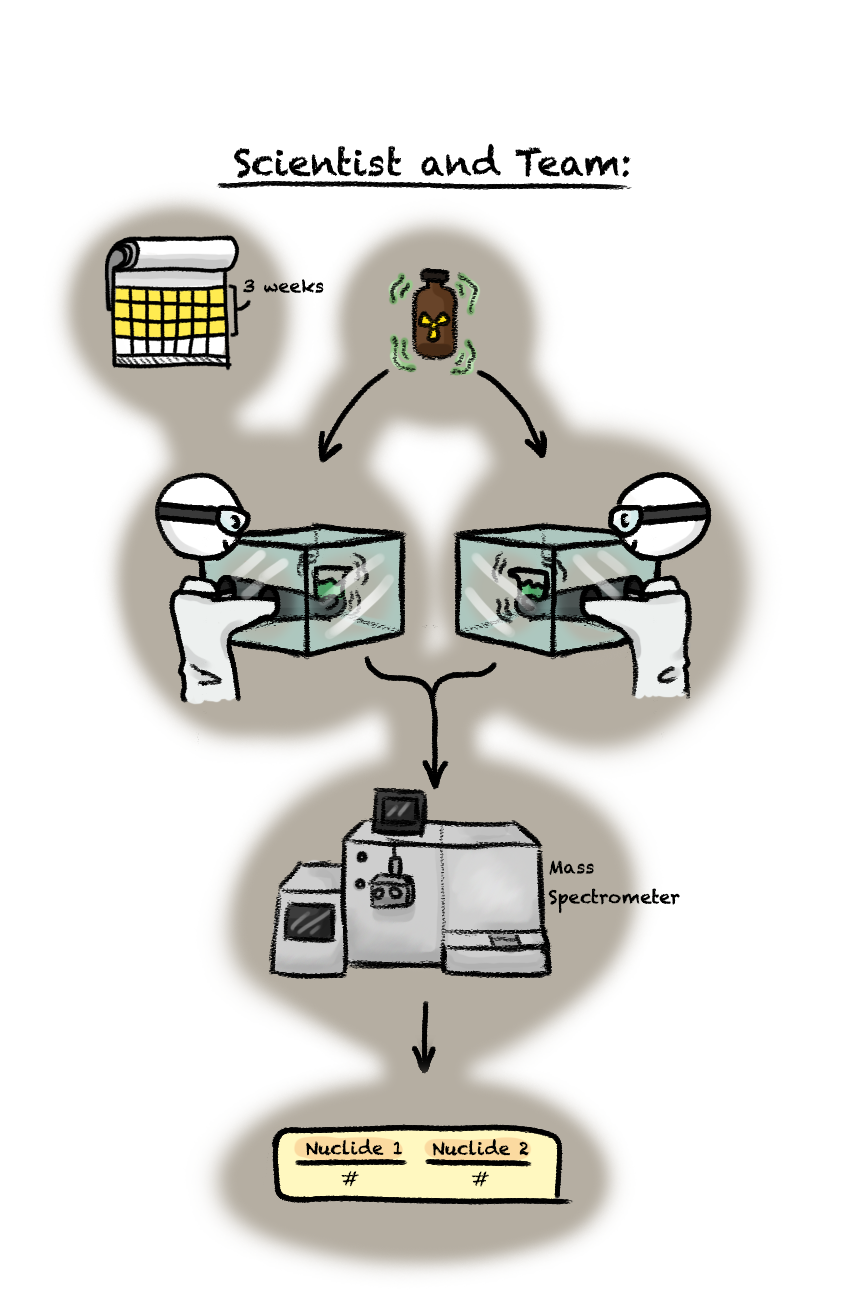
\includegraphics[width=1.2\linewidth]{./chapters/public/mass_spec.png}}
      \large This process is complicated, but here are some snapshots. 
      \small Illustration by Anna Stephenson
    \end{figure}
    \vspace{-7mm}
    
    Now they were ready to borrow our friend's machine
    learning method to predict the parameters of the reactor operation history.
    The scientist then took the list of 29 nuclides and their measurements and
    compared that information against their machine-learned model that was
    created using a training set composed of $450,000$ of the exact same 29
    simulated measurements of different types of nuclear fuel. And out popped
    an answer:
    
  \end{minipage}
}

\begin{tcolorbox}[halign=center]
\textbf{Results}
\end{tcolorbox}
\vspace{-4mm}

\fcolorbox{gray!10}{gray!10}{
  \begin{minipage}[t]{0.45\textwidth}
    
    \setlength{\parskip}{1em}
    
    \begin{table}[H]
      \centering
      \begin{tabular}{ll} \toprule
        Reactor Type     & BWR                          \\
        Burnup           & 44.02 $\scriptstyle GWd/MTU$ \\
        Enrichment       & 2.04 \%\:${}^{235}\text{U}$  \\
        Time Since Irrad & 5.34 $years$                 \\ \bottomrule
      \end{tabular}
    \end{table}
    \vspace{-2mm}
    
    ``Ok! We got it!'' said our friend. Given these values, some of the UFU
    authorities specializing in worldwide reactor operational history databases
    were able to determine this came from a reactor in the Democratic People's
    Republic of Thoria (DPRT). 
    
  
    This made sense to everyone because the DPRT had been a threat for some
    time. Everyone knew their missiles couldn't get to the UFU, so they must
    have concocted a different plan.

    It was a matter of hours before the UFU had hundreds of DPRT conspirators
    in custody. With the culprits contained, the drone-delivered material
    didn't make it to the bomb assembly location, and the day was saved!
    
    \ldots Except, three weeks later, the capital city of Curiumville was
    bombed.
  
  \end{minipage}%
}
  \hfill\vline\hfill
\fcolorbox{gray!10}{gray!10}{
  \begin{minipage}[t]{0.45\textwidth}
    
    \setlength{\parskip}{1em}
  
    \begin{table}[H]
      \centering
      \begin{tabular}{ll} \toprule
        Reactor Type     & BWR                          \\
        Burnup           & 44.02 $\scriptstyle GWd/MTU$ \\
        Enrichment       & 4.11 \%\:${}^{235}\text{U}$  \\
        Time Since Irrad & 4.65 $years$                 \\ \bottomrule
      \end{tabular}
    \end{table}
    \vspace{-2mm}

    ``Ok! We got it!'' said the scientist. Given these values, some of the UFU
    authorities specializing in worldwide reactor operational history databases
    were able to determine this came from a reactor in \ldots GASP! 

    The Commonwealth of Puerto Plutonio, a Territory of the UFU?! This made no
    sense! We thought they liked being colonized!

    It was now a rush to track down the conspirators since there wasn't much
    intelligence data on them. The UFU was scrambling. 

    And in the middle of the scramble, the capital city of Curiumville was
    bombed.
  
  \end{minipage}
}

\vspace{4mm}

\narr Now, curious companion, you are both permitted and encouraged to read the
other adventure. 

After weeks went by the UFU authorities with the help of the scientist were
able to confirm the actual parameters:
\vspace{8mm}
\begin{table}[H]
  \centering
  \begin{tabular}{ll} \toprule
    Reactor Type           & BWR                         \\
    Burnup                 & 44.02 $GWd/MTU$             \\
    Enrichment             & 4.11 \%\:${}^{235}\text{U}$ \\
    Time Since Irradiation & 4.86 $years$                \\ \bottomrule
  \end{tabular}
\end{table}

Our friend's experimental machine learning method isn't so bad! The scientist's
mass spectrometry-based approach almost gave correct answers for all four
parameters; the time since irradiation was off by 2-3 months.  Our friend's
gamma spectroscopy-based approach predicted the correct reactor type and
burnup, but the time since irradiation was 6 months too long. Most
significantly, though, it could not predict the proper \gls{U235} enrichment,
and this is what led to the false blame on the DPRT.  

In both versions, luckily, the bomb didn't detonate and no one died. It was too
rushed of a job, and with the nuclear test ban treaty, no one actually knows
their nuclear weapons WILL work. You didn't think our friend's tale was going
that dark, did you?

\vspace{8mm}
\begin{shadequote}

  ``Hey,'' the scientist said to our friend, ``I'm famished.'' Our friend said, ``Oh
  goodness, me too!'' They looked at each other, and after some telepathic
  decision making, agreed on a nice steak.

\end{shadequote}

\begin{figure}[H]
  \centering
  \makebox[\textwidth][c]{
\includegraphics[width=0.75\linewidth]{./chapters/public/theend.png}}
  \large The end. \small Illustration by Anna Stephenson \\~\\
\end{figure}

\hrule

\begin{tcolorbox}[halign=center]
\textbf{Discussion \& Conclusions}
\end{tcolorbox}

This machine learning-based research protocol is designed to answer the
question: \textit{How does the ability to determine forensic-relevant spent
nuclear fuel attributes using machine-learning techniques degrade as less
information is available?} The dissertation written after this chapter answers
that in much more detail than the two scenarios presented here, but I hope to
have communicated the basics of what I'm doing to a general audience. I
actually don't use any real-measured samples by which to compare the different
types of training sets (the samples in this story are a part of my work, but
simulated), but I do use a real-world set of test cases with the 29 nuclide
mass training set.  There are many challenges with doing this yet to be
resolved, so it is not presented here in a research snapshot.

The lack of a feel-good resolution in this tale is not meant to reduce
confidence in our national nuclear forensics capability or my research project,
but rather to show how science does not necessarily result in clear-cut answers
to questions. Much of the time, asking a question and answering it using the
scientific method creates more questions than answers. For example,  there are
questions about why the gamma spectra approach gave such a wrong enrichment
prediction (something echoed in my results, which are aggregate statistics of
$450,000$ cases versus the one case presented here). Another question might be
whether a 3-month or 6-month time since irradiation error prediction is too
large of an error, or an acceptable error.

\begin{tcolorbox}[halign=center]
\textbf{Author Commentary}
\end{tcolorbox}

\textit{Last, I wanted to make a short statement about my work on an even
broader scale.}

Every scientist should take note of the ethical and political implications of
their work. Yes, I said it: science is political\footnote[8]{Everyone knows
\href{https://www.scientificamerican.com/article/yes-science-is-political/}{\color{violet}it}!}!
Although the morality of preventing or mitigating a nuclear disaster is not
necessarily in question, the nuclear field (both commercial power and
defense/the nuclear weapon program) is far from blameless when it comes to
destroying human bodies and the environment. The mining industry caused uranium
contamination and early death for many Din\'{e} in Navajo Nation and
payouts/cleanup only began recently\footnote[9]{For more information about the
500 abandoned mines and the cleanup efforts, read more
\href{https://www.epa.gov/navajo-nation-uranium-cleanup/abandoned-mines-cleanup}{\color{violet}here}.},
plutonium production during World War II has resulted in the displacement and
illness of US citizens around Hanford, WA, and government-sanctioned human
radiation experiments were conducted on unwitting people and children. None of
this (and so much more that's not mentioned here) comes as a surprise knowing
the entire nuclear enterprise sits on a foundation of well-documented
racism\footnote[10]{\href{https://thebulletin.org/2020/08/a-call-for-antiracist-action-and-accountability-in-the-us-nuclear-community/}{\color{violet}Here's}
a good article on nuclear's racist roots.}.  Last, the obvious must be stated:
the US is the only country to ever deploy a nuclear weapon against another
country, where the human toll was undeniably brutal\footnote[11]{And Black
American journalists
\href{https://www.nytimes.com/2021/08/09/science/charles-loeb-atomic-bomb.html?smid=url-share
}{\color{violet}exposed the government's lies} about it}. This and much more is
documented in a list of resources curated by Kalin Kiesling with help from the
nuclear community\footnote[12]{The resources are curated in
\href{https://docs.google.com/document/d/e/2PACX-1vQuRSix5J31G4yhH-Z0kwmlpXe6OgS9MXg6l-LBEOVNDPDAPVivPSrJ7A71TMCsW2EdvGMepZCcwdTP/pub}{\color{violet}this
Google document}.}.

None of this means that nuclear power as an energy source is inherently evil,
but the industry and our government must acknowledge and take responsibility
for abusing both the land and the beings on it. It is hard to hold this
knowledge and still want to participate in nuclear science, but if more people
in nuclear science and industry also hold this knowledge, then maybe taking
life and land for granted can be less of a norm. Of course, better policy is
always a stronger influence. Why am I saying all of this inside a(n unofficial)
chapter in a nuclear engineering dissertation? Science is political, and so I
must be too.  

}
